\documentclass[12pt,a4paper]{article}
    \usepackage[T2A]{fontenc}
    \usepackage[utf8]{inputenc}
    \usepackage[russian]{babel}
    \usepackage{amsmath}
    \usepackage{amssymb}
    \usepackage{graphicx}
    \usepackage{floatrow}
    \usepackage{booktabs}
    \usepackage{wrapfig}
    \usepackage{lipsum}
    \usepackage{subcaption}
    \usepackage{fancyhdr}
    \usepackage{mathrsfs}
    \usepackage{tikz}

    \usepackage{graphicx, scalerel}
    \usepackage[warn]{mathtext}
    \usepackage{indentfirst}
    \usepackage[margin = 25mm]{geometry}
    \usepackage{caption}
    \usepackage{multirow}
    \usepackage{gensymb}
    
    \newcommand{\figref}[1]{(См. рис. \ref{#1})}
    \newcommand{\secref}[1]{(См. раздел. \ref{#1})}
    
    \newcommand{\e}[1]{\text{$\cdot10^{#1}$}}
    
    \pagestyle{fancy}
    \fancyhead{}
    \fancyhead[L]{Работа 5.10.1}
    \fancyhead[R]{}
    \fancyfoot[C]{\thepage}
    
    \author{\normalsize Выполнил: Голубович Тимур, группа Б01-110 \\
    	\normalsize 08.11.2023}
    \date{}

    \usepackage{float}
    \restylefloat{table}
    \title{
    	\large Отчет о выполнении лабораторной работы 5.10.1 \\
    	\Large Электронный парамагнитный резонанс
     }

    \begin{document}
\maketitle

\section*{Цель работы}

Исследовать электронный парамагнитный резонанс в молекуле ДФПГ, определить $g$-фактор электрона, измерить ширину ЭПР.


\section*{Оборудование и приборы}

Источник  $\gamma$-квантов со свинцовым коллиматором; набор поглотителей из различных материалов; сцинтилляционныйй счётчик; пересчётный прибор.
	
\section*{Теоретическое введение}

Энергетический уровень электрона в присутствии магнитного поля с индукцией $B$ расщепляется на два подуровня, расстояние между которыми равно 

\[	\Delta E = E_2 - E_1 = 2\mu B_0.\]
    
Здесь $\mu$ -- абсолютная величина проекции магнитного момента на направление поля.

Между этими двумя уровнями возможны переходы. Эти переходы могут возбуждаться внешним высокочастотным электромагнитным полем, если оно имеет нужную частоту и нужное направление.

Резонансное значение частоты определяется из очевидной формулы:

\[	\hbar \omega_0 = \Delta E.\]

При переходе с нижнего на верхний уровень энергии электрон поглощает квант электромагнитной энергии, а при обратном переходе такой же квант излучается. Возбуждение электронных резонансных переходов электромагнитным полем, имеющим частоту $\omega_0$, носит название электронного парамагнитного резонанса (ЭПР).

В настоящей работе необходимо получить сигнал ЭПР на кристаллическом дифенилпикрилгидразиле (ДФПГ) и определить значение $g$-фактора для электрона. Как известно, связь между магнитным моментом $\mu$ электрона и его механическим моментом $\mathbf{M}$ выражается через гиромагнитное отношение $\gamma$ с помощью формулы

\[ \mu = \gamma M.\]

Если магнитный момент частицы измерять в магнитонах Бора, а механический - в $\hbar$, то их связь можно записать через $g$-фактор:

 \[ \frac{\mu}{\mu_\text{Б}} = g \frac{M}{\hbar} = g \frac{s\hbar}{\hbar} = gs = \frac{\hbar \omega_0}{2 B_0 \mu_\text{Б}}\]

,где $s = 1/2$ -- спин электрона

Значит g-фактор:

\[	g = \frac{\hbar \omega_0}{\mu_\text{Б} B_0}.\]
 
\section*{Экспериментальная установка}
	
Схема экспериментальной установки приведена на рис.1.

\begin{figure}[H]
  \begin{center}
    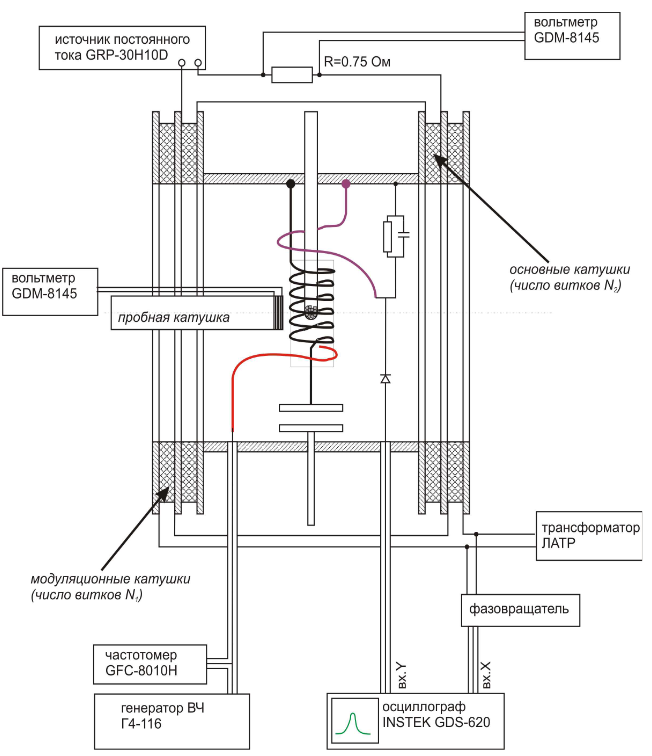
\includegraphics[width=10cm]{res/scheme.png}
    \caption{Схема экспериментальной установки.}
    \label{fig:}
  \end{center}
\end{figure}
 
	
Схема установки представлена на Рис. 1. Образец (порошок ДФПГ) в стеклянной ампуле помещается внутрь катушки индуктивности, входящей в состав колебательного контура. Входящий в состав контура конденсатор состоит из двух пластин, разделённых воздушным зазором, одна из пластин может перемещаться поворотом штока. Колебания в контуре возбуждаются антенной, соединённой с генератором высокой частоты (ВЧ) Г4-116. Амплитуда колебаний поля в катушке индуктивности
измеряется по наводимой в петле связи ЭДС индукции. Высокочастотные колебания ЭДС
индукции в приёмном контуре детектируются диодом, измеряемая при помощи
осциллографа низкочастотная огибающая этого сигнала пропорциональна квадрату
амплитуды колебаний поля в катушке.\\
Постоянное магнитное поле создаётся пропусканием тока от источника постоянного тока через основные катушки. 

\section*{Ход работы}

\textbf{Характеристики пробной катушки}

  \begin{table}[H]
\begin{center}
\begin{tabular}{|c|c|}
\hline N, \text{шт} &D, mm\\
\hline 49& 14.3\\
\hline
\end{tabular}
\end{center}
\end{table}
 
 \begin{enumerate}
    \item \textbf{Настройка ВЧ генератора на частоту колебательного контура.} Подстройкой частоты добиваемся максимальной амплитуды сигнала на экране осциллографа. Эта частота равна $f_0 =$124.0 МГц. Осциллограмма при настройке генератора изображена на рис.2.
        		    \begin{figure}[H]
  \begin{center}
    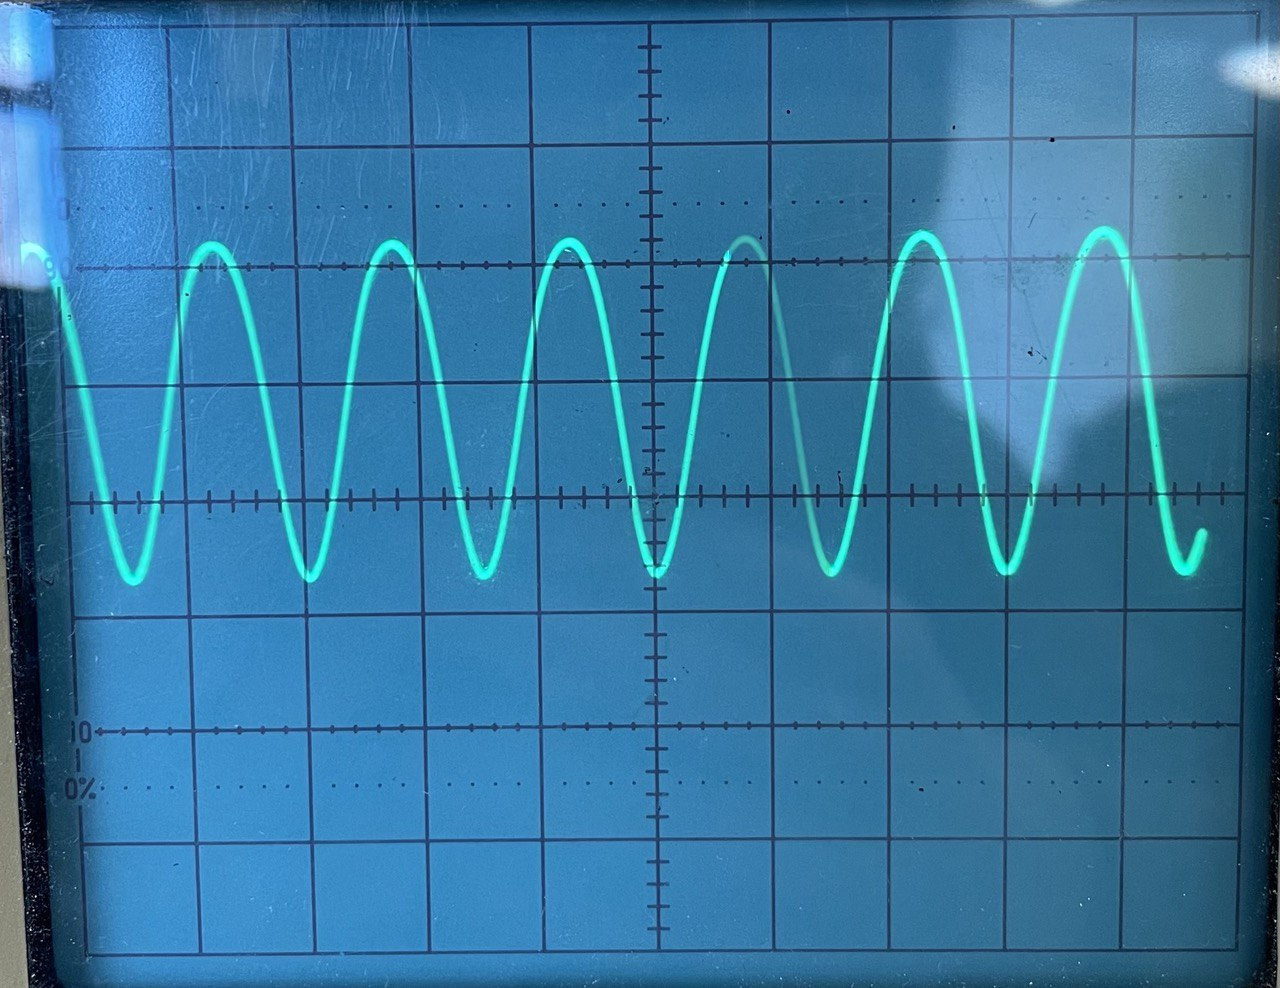
\includegraphics[width=12cm]{src/ex2.jpg}
    \caption{Осциллограмма при настройке генератора.}
    \label{fig:}
  \end{center}
\end{figure}

    \item \textbf{Наблюдение сигнала резонансного поглощения.} Для этого подключаем основные катушки к источнику постоянного тока, а модуляционные катушки к трансформатору ЛАТР. Подбираем величину постоянного магнитного поля в основных катушках так, чтобы наблюдался сигнал резонансного поглощения. Добиваемся эквидистантности пиков. 
  \newline 
  
  Зафиксированный сигнал изображен на рис. 3.
    
       		    \begin{figure}[H]
  \begin{center}
    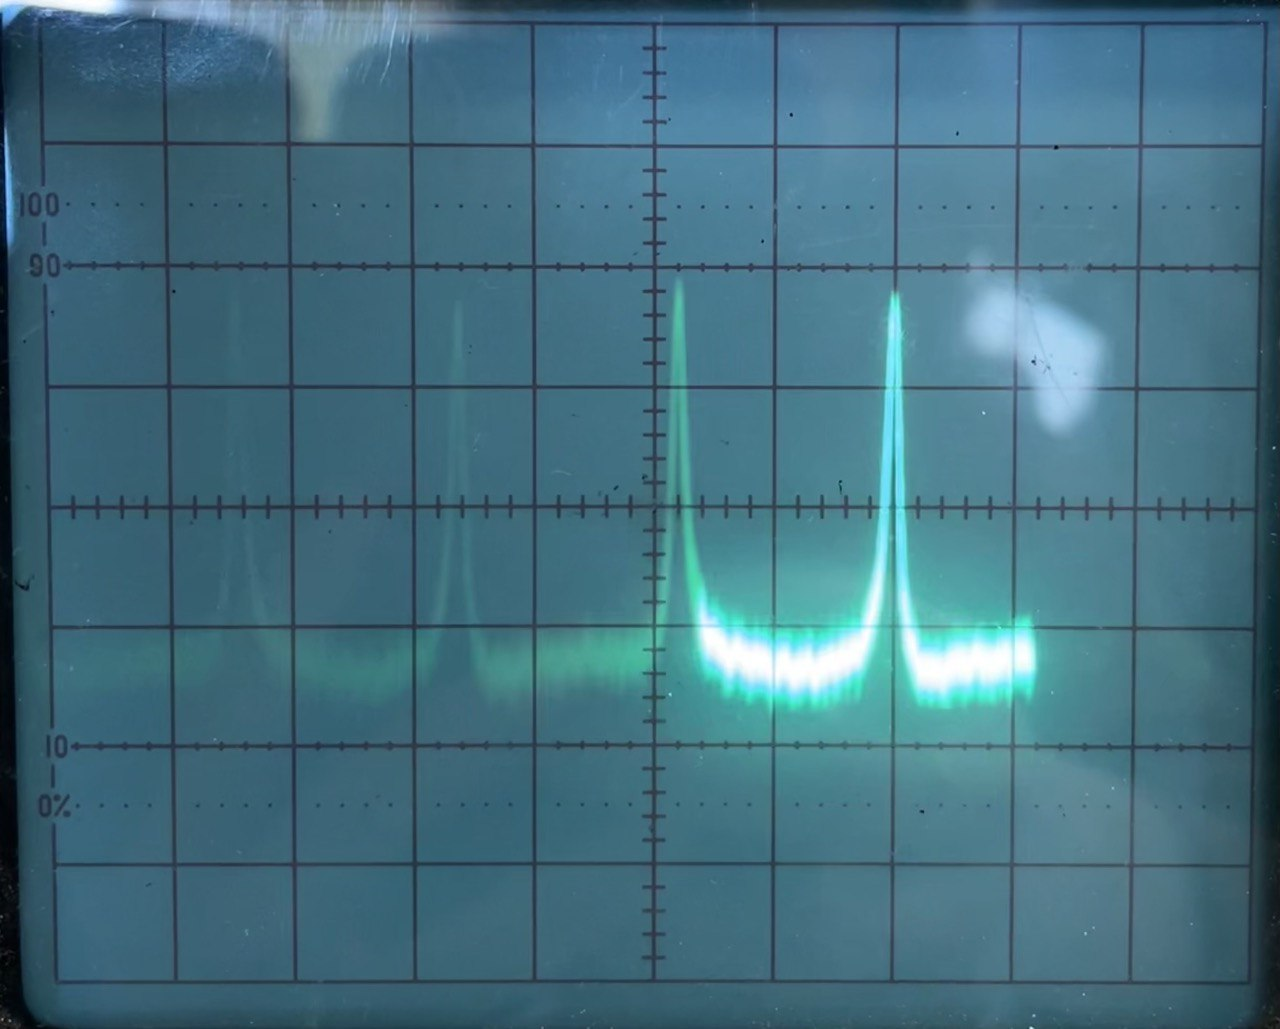
\includegraphics[width=12cm]{src/ex3.jpg}
    \caption{Осциллограмма сигнала поглощения при резонансном постоянном поле.}
    \label{fig:}
  \end{center}
\end{figure}
    
    Вносим пробную катушку в соленоид и измеряем ЭДС-индукции:
    
    $U = (11.14 \pm 0.01)$ мВ
    
    По этой величине можем рассчитать величину постоянного магнитного поля:
    
    \[U = N_{\text{проб}} S \omega B_0 =>  B_0 = \frac{U}{N_{\text{проб}} S \omega} = (4.51 \pm 0.01) \text{мТл}\]
    
    , где $S = \frac{\pi (D_{проб})^2}{4}$-- площадь сечения пробной катушки, $\omega = 2\pi \vartheta $ -- угловая частота переменного тока, $\vartheta $= 50 Гц.
    
 
% Это комментарий
%    		    \begin{figure}[H]
%  \begin{center}
%    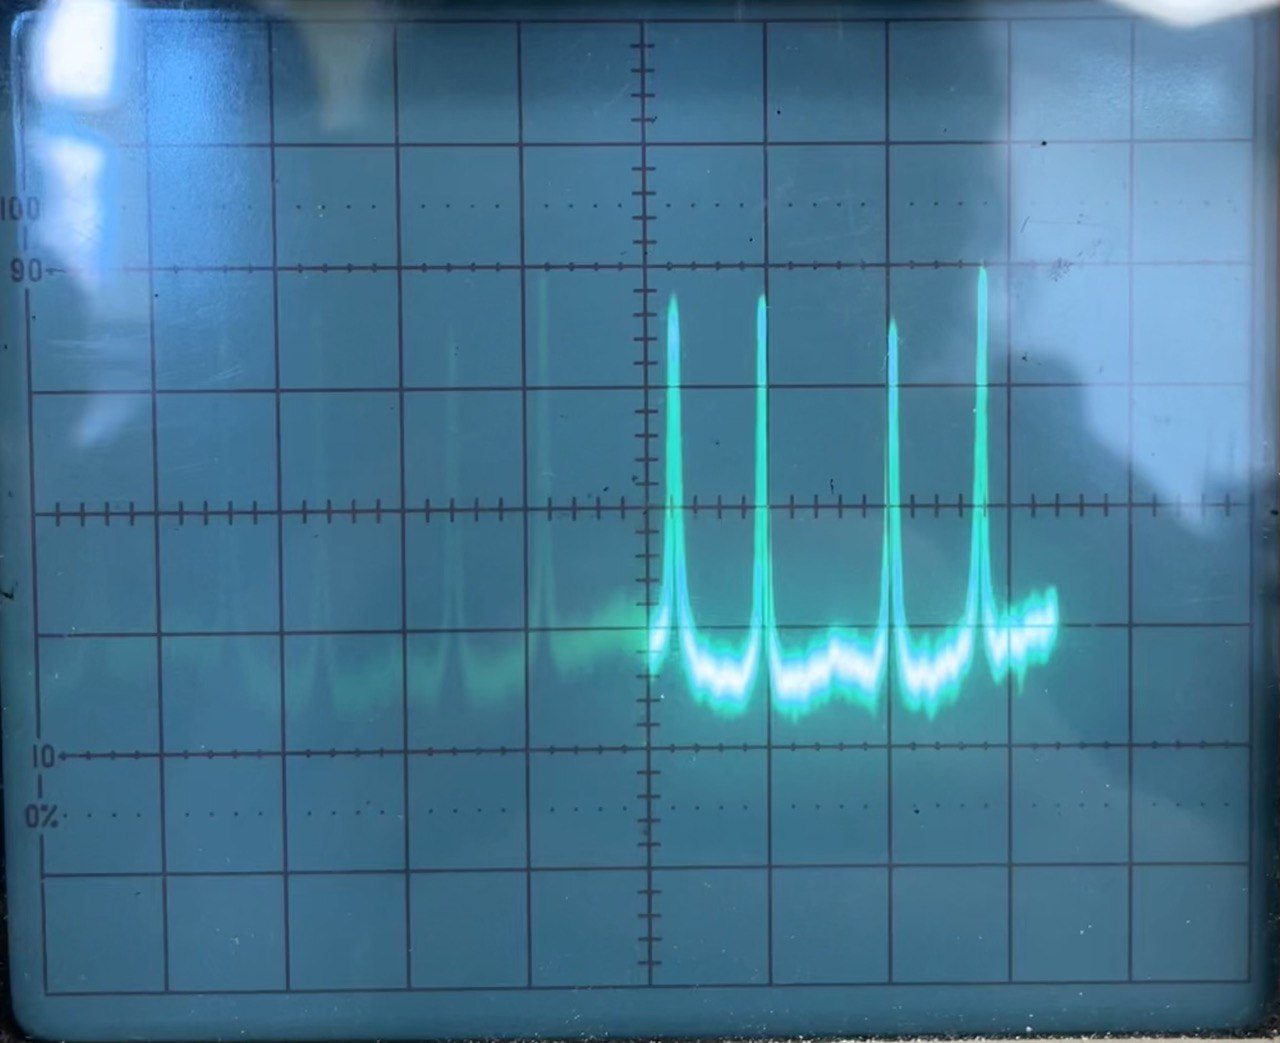
\includegraphics[width=12cm]{ex4.jpg}
%    \caption{А здесь в два раза чаще.}
%    \label{fig:}
%  \end{center}
%\end{figure}

   \item \textbf{Определение ширины линии поглощения.} Переводим осциллограф в режим XY-развертки.
   
    
   \textbf{X} - напряжение на модулирующих катушках
   
   \textbf{Y} - сигнал с детектора
   
   Добиваемся появления хорошо прорисованной линии резонансного поглощения. Подстройкой фазовращателя совмещаем два пика, соответствующих прохождению резонансного поглощения на растущем и падающем полупериодах модулирующего напряжения. Наблюдаемый сигнал изображен на рис.5. 
   
         \begin{figure}[H]
  \begin{center}
    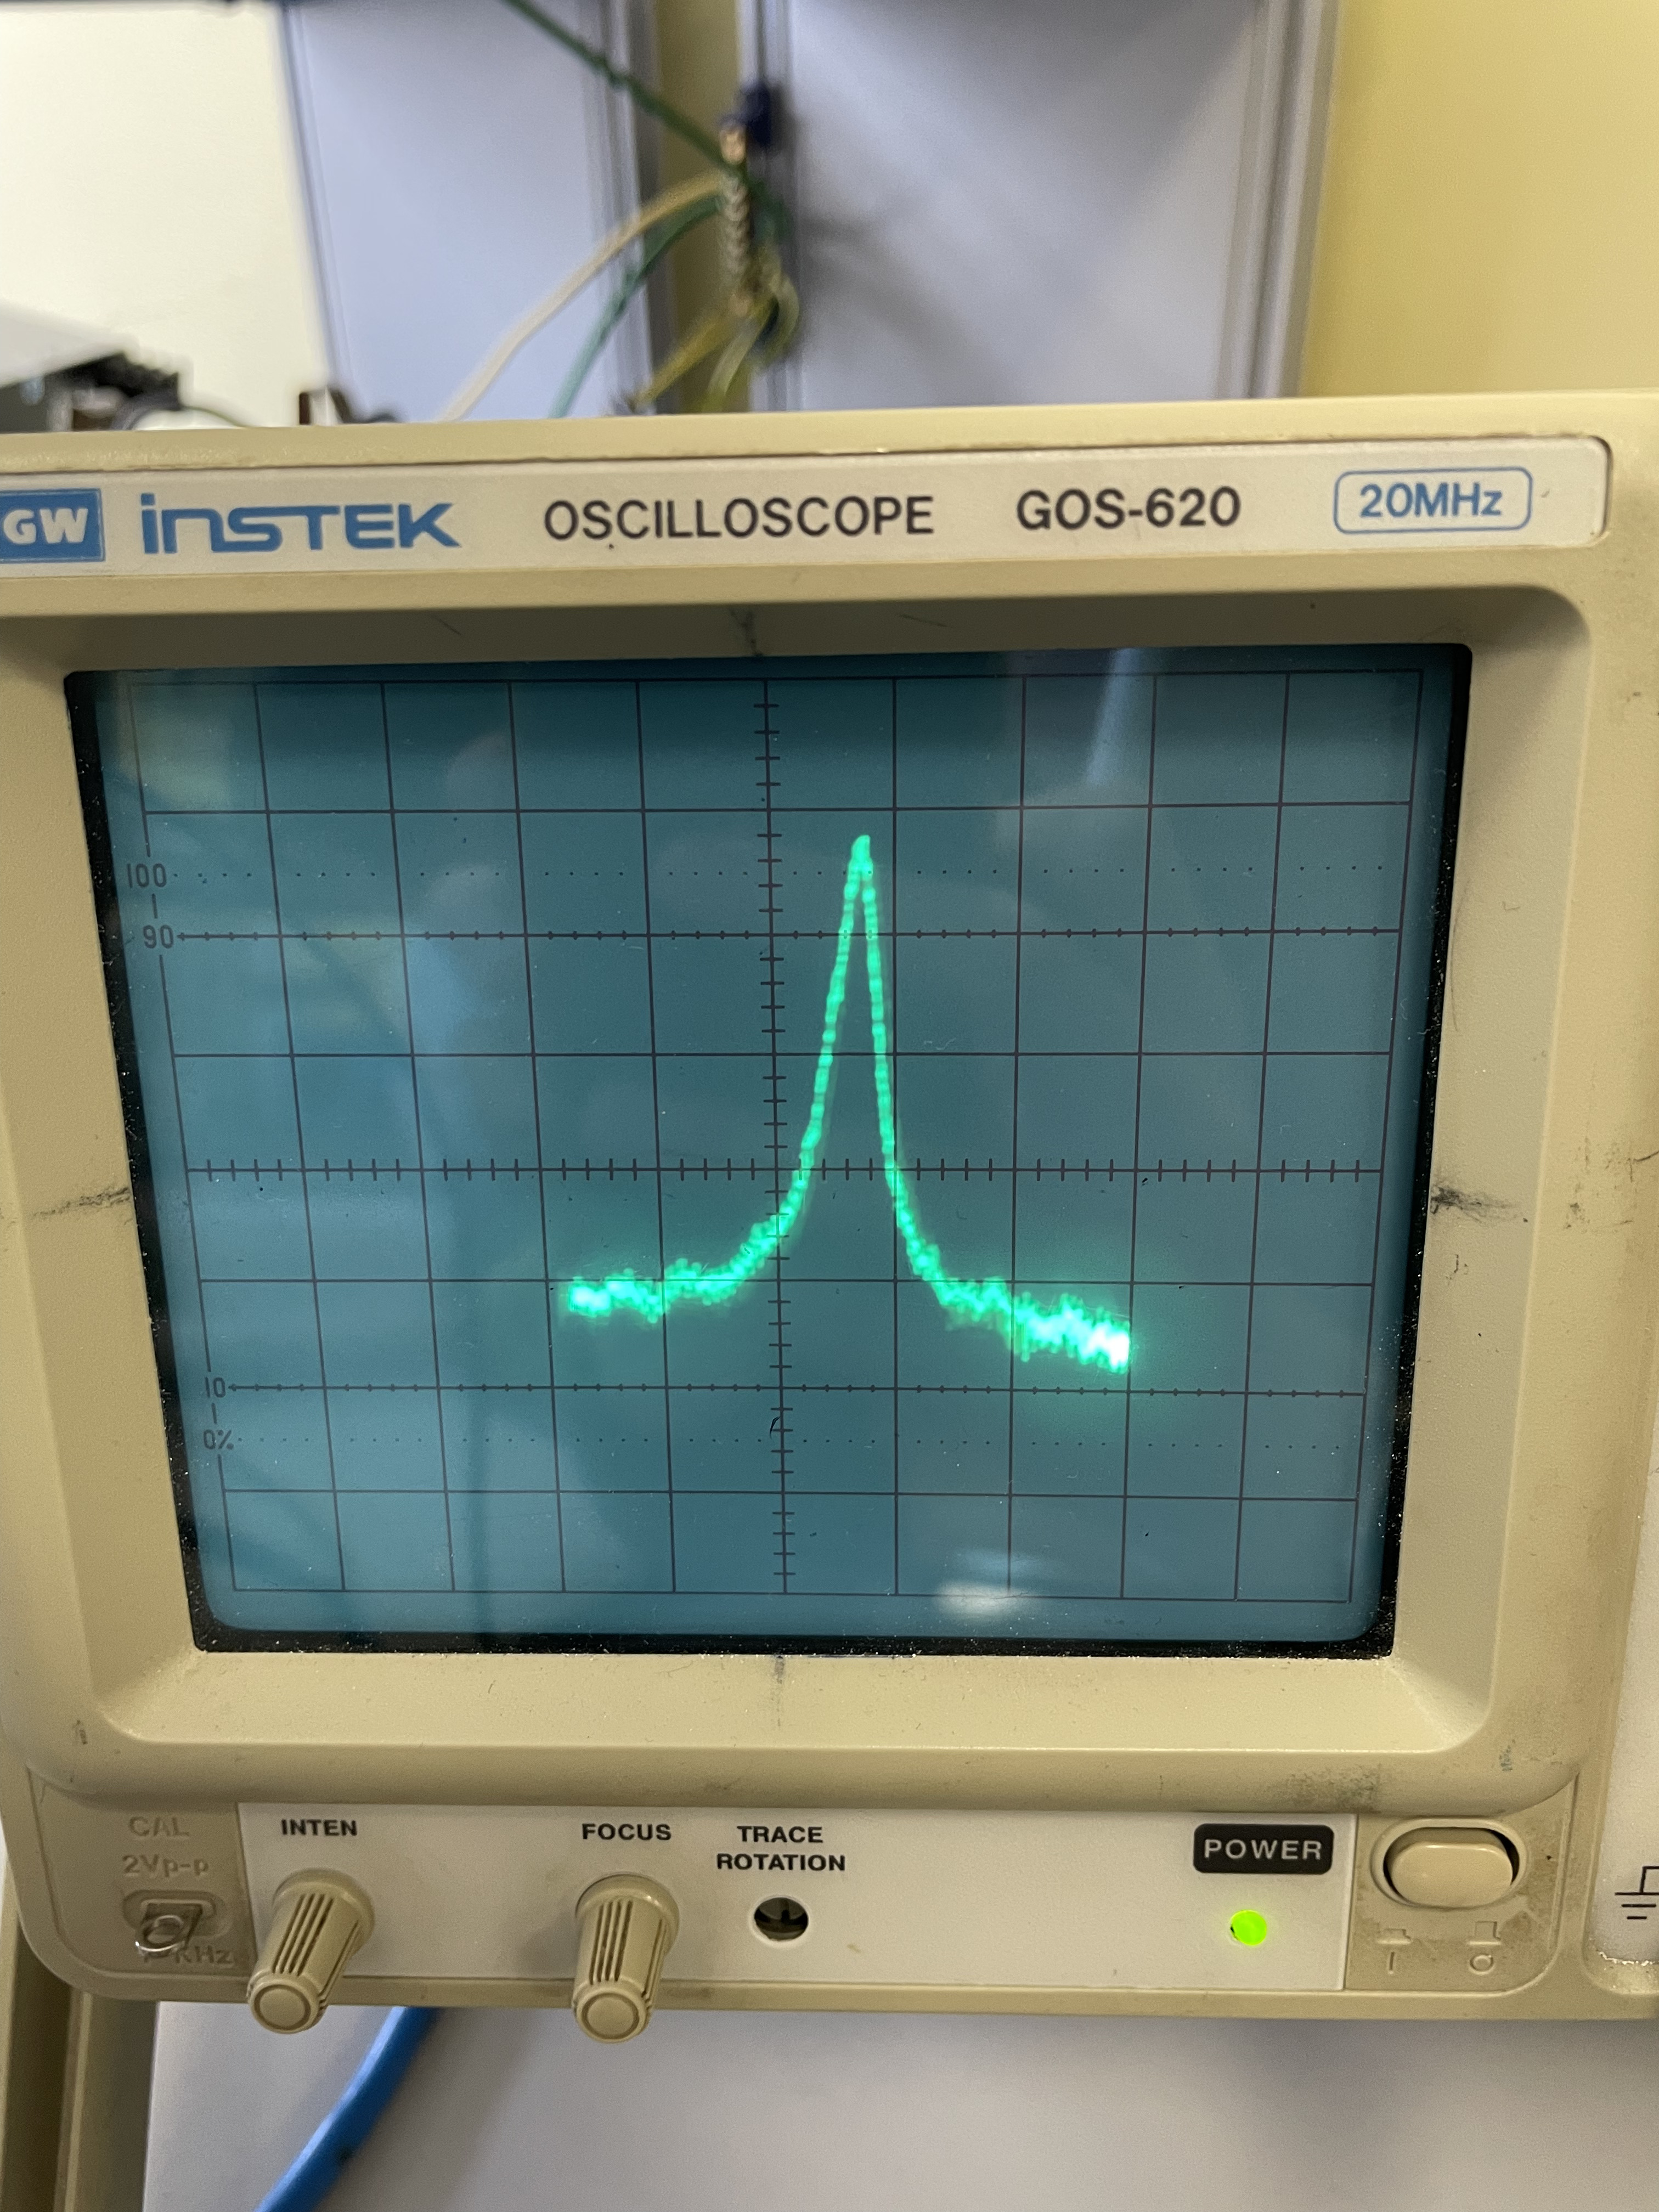
\includegraphics[width=12cm]{src/ex5.jpg}
    \caption{Линия резонансного поглощения в режиме XY-развертки.}
    \label{fig:}
  \end{center}
\end{figure}

   
    \item Для определения ширины линии ЭПР определим по экрану осцилографа полный размах поля $A_{0}$ и полную ширину кривой резонансного поглощения на полувысоте $A_{\frac{1}{2}}$. 
    
    $A_{0} = 6.0 \pm 0.2 $дел
    
    $A_{\frac{1}{2}} = 0.6 \pm 0.2$ дел
    
    При помощи пробной катушки определим амплитуду модуляции магнитного поля. Для этого внесем её внутрь соленоида. Переменное поле модуляционных катушек наводит в пробной катушке ЭДС индукции $\varepsilon $, по которой можно определить величину поля. Измеренное ЭДС индукции: 
    
    $\varepsilon = (3.21 \pm  0.01)$мВ
    
     \textbf{Амплитуда модулирующего поля}:
    
    $B_{\text{мод}} = \dfrac{2\sqrt{2} \varepsilon }{\pi^2 d^2_{\text{проб}} N_{\text{проб}}\vartheta } = (1.84 \pm 0.01)$ мТл
    
    , где $\vartheta $= 50 Гц -- частота модулирующего напряжения 


  Тогда  \textbf{ширина линии ЭПР}:
  
  $\Delta B = \frac{A_{\frac{1}{2}}}{A_{0}} B_{\text{мод}} = (0.18 \pm 0.06)$ мТл
    
    
		\item \textbf{Определение $g$-фактора}. По полученным данным определяем значение эффективного $g$-фактора исследуемого вещества ($\hbar = 1.054 \cdot 10^{-34} \text{Дж с}, \mu_\text{Б} = 927.4 \cdot 10^{-26} \text{Дж/Тл}$):
		
		\[g = \frac{\hbar \omega_0}{\mu_\text{Б} B_0} = \frac{\hbar 2 \pi f_0}{\mu_\text{Б} B_0} = (1.96 \pm 0.01)\]

	
\textbf{Табличное значение} g-фактора свободного электрона - $g_{\text{своб}} = 2.0036$. Отклонение от табличного значения - 1\%.
	\end{enumerate}


\clearpage
    
\section*{Вывод}

В данной работе мы исследовали ЭПР в молекуле ДФПГ. Измерили 

\textbf{Ширину линии резонансного поглощения}, ее значение составило $\Delta B = 0.18$ мТл. 

\textbf{g-фактор электрона}, значение которого составило g = 1.96. Данное значение совпадает с точностью 1\% с табличным значением для свободного электрона $g_{\text{своб}} = 2.0036$, это свидетельствует о том, что ЭПР происходит на неспаренных электронах почти так же, как и на свободных.


\begin{itemize}
    \item фотоэффект (пики полного поглощения)
    \item эффект Комптона (характерное распределение энергий в спектре, оканчивающееся комптоновским краем)
    \item обратное рассеяние (пики обратного рассеяния)
    \item аннигиляция позитронов (пик 511 keV в спектре натрия, по которому проводилась калибровка)
\end{itemize}

Все значения энергии, опеределённые по спектрам, практически совпадали с табличными и расчётными. \par

Также была проверена линейная зависимость квадрата спектрального разрешения прибора от величины, обратной энергии полного поглощения.

\vfill
    
\begin{thebibliography}{9}
	\bibitem{max} \emph{Лабораторный практикум по общей физике. В 3 томах. Том 3. Квантовая физика: учебное пособие} под ред. Ю. М. Ципенюка
\end{thebibliography}

\end{document}
